
%!TEX root = Main.tex
\documentclass[Main]{subfiles}

\begin{document}

\section{Robot Mechanics} % (fold)
	\label{sec:robot_mechanics}

	\subsection{Chassis} % (fold)
		\label{sub:chassis}
		The chassis of the robot is a Baron-4WD mobile platform bought from the website dfrobots.com. It consist of a lower frame where up to four DC motors can be attached, and a top plate with holes for mounting of other devices. \autoref{fig:baron_platform} show a picture of the chassis where it is assembled with the default package items from dfrobots.
\begin{figure}[H]
	\centering
	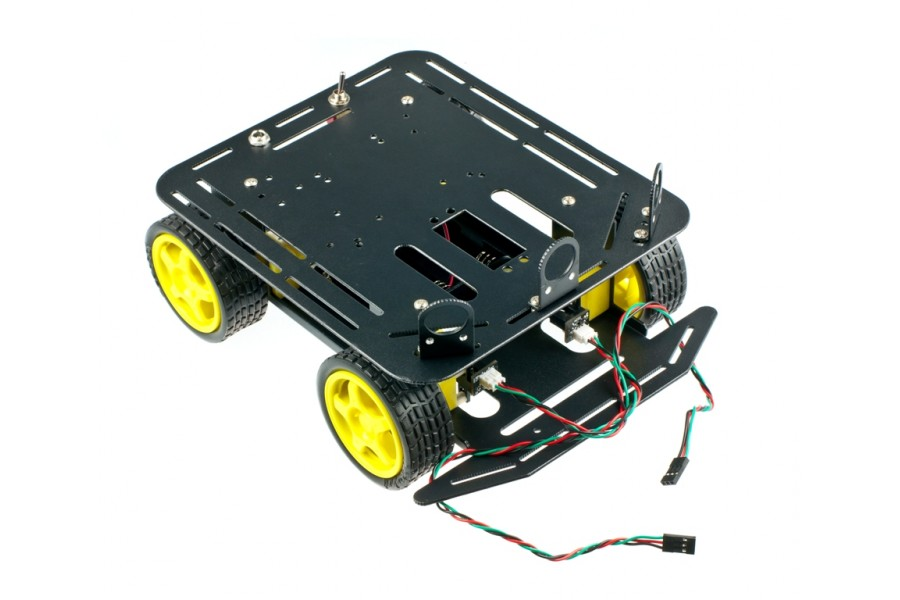
\includegraphics[scale=0.5]{./Figures/baron_platform.jpg}
	\caption{The Baron-4WD platform}
	\label{fig:baron_platform}
\end{figure}\noindent
In this project it was decide to only use two motors at the rear end of the chassis to make a simpler motion model for the robot; more about the motion model in \autoref{sub:motion_model}. Instead of front wheels, a ball caster was attach to insure the turning ability. By only using motors in the rear end, the lower frame had a lot of room where the power supplies could be place and thereby leaving the top plate free for the processing platform, a Zybo development board \fxnote{ref}, and mounting of the sensors. The sensor used in this project was a LIDAR \fxnote{ref} which required a specific mounting pattern, that filled out most of the top plate's area, thereby only leaving a small area for the Zybo board. The LIDAR was therefore mounted on a acrylic plate which then was mounted on top of the top plate. The final robot configuration is shown in \autoref{fig:final_robot}.
\begin{figure}[H]
	\centering
	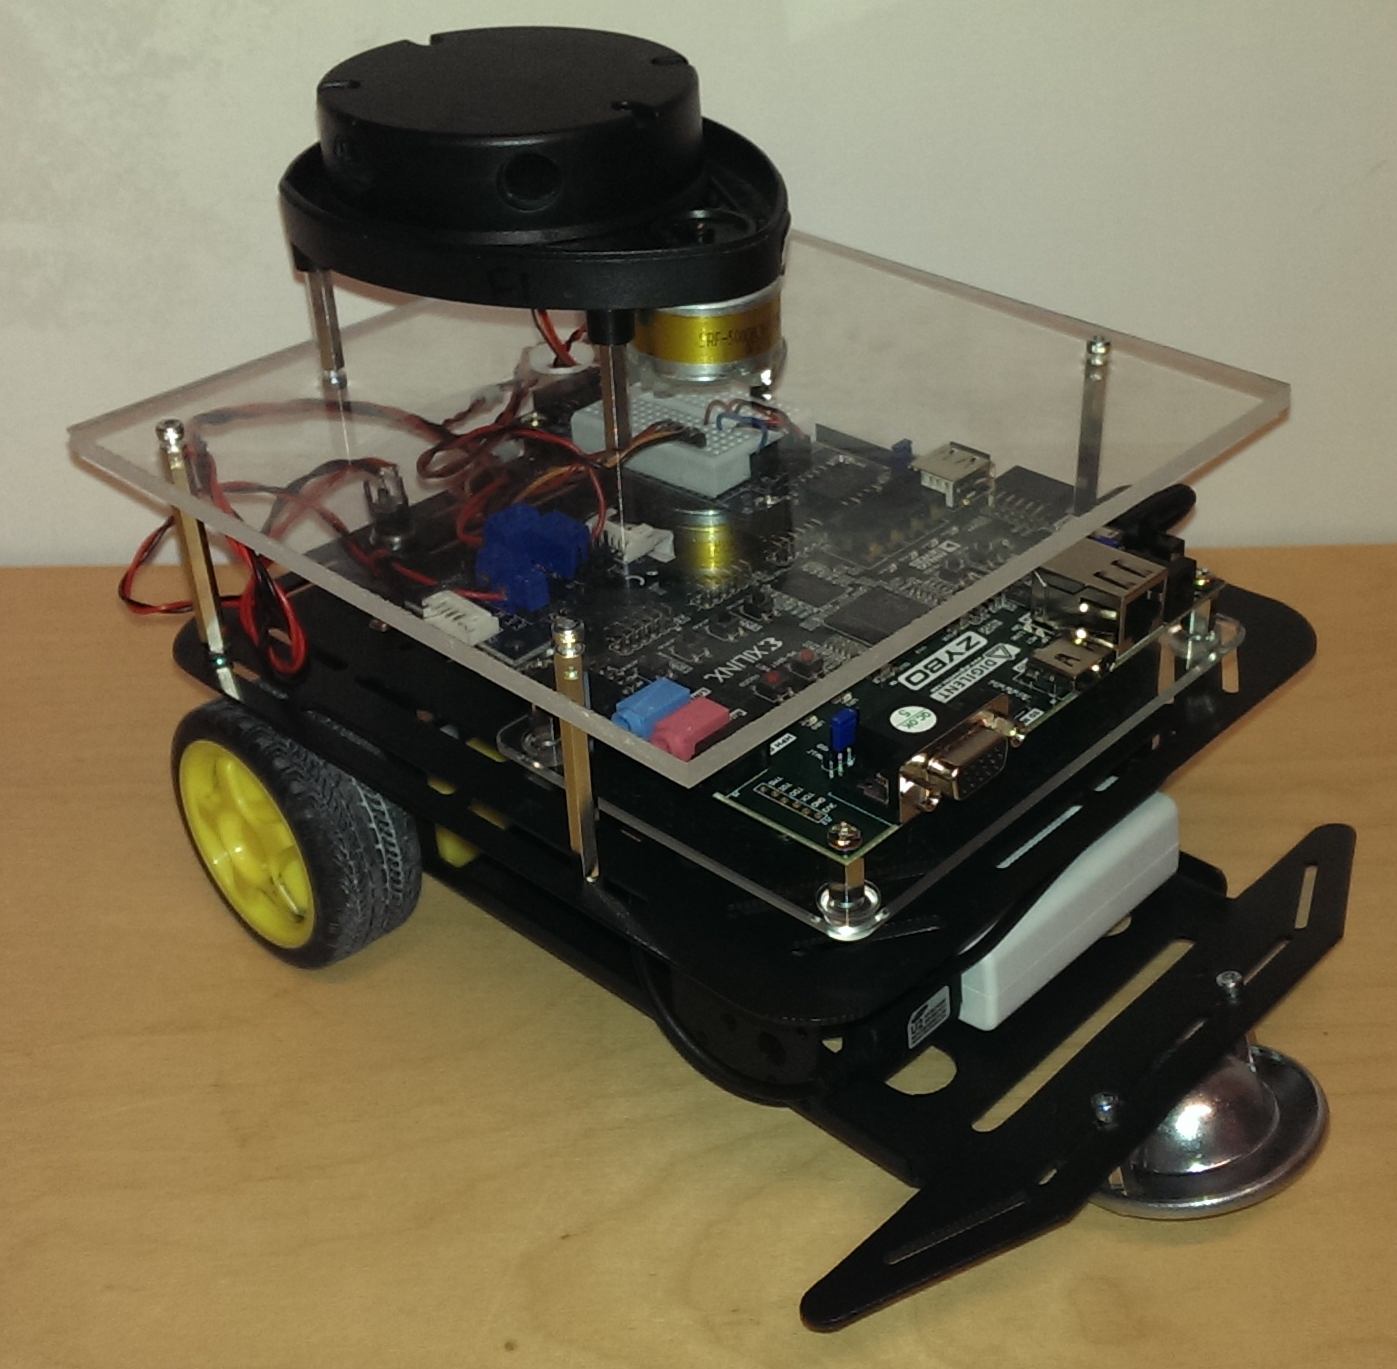
\includegraphics[scale=0.3]{./Figures/final_robot.png}
	\caption{The final robot configuration}
	\label{fig:final_robot}
\end{figure}\noindent
		% subsection chassis (end)

	\subsection{Motor characteristics} % (fold)
		\label{sub:motor_characteristics}
		
		% subsection propulsion (end)

	\subsection{Motion model} % (fold)
		\label{sub:motion_model}
		
		% subsection motion_model (end)

	% subsection robot_mechanics (end)

\end{document}